\section{Zielsetzung}
Ziel der Versuch ist es die elastischen Konstanten eines Körpers (hier: einer Kugel) zu bestimmen. Anschließend soll das magnetische
Moment eines Permanentmagneten unter Zuhilfenahme eines Helmholtzspulenpaares bestimmt werden.
\section{Theorie}
\label{sec:Theorie}
    \subsection{Normal- und Schubspannung}
    Wenn auf die Oberfläche eines Körpers eine Kraft $F$ wirkt, kann es dabei zu Verformungen und Volumenänderungen am Körper
    kommen. Hier soll $F$ eine Zugkraft sein, das heißt eine Kraft die an der Oberfläche des Körpers \"zieht\". Diese Kraft wird
    als Spannung bezeichnet, wobei die auf der Oberfläche senkrechtstehende Komponente als Normalspannung $\sigma$ bezeichnet wird
    und die Komponente welche parallel zur Oberfläche verläuft als Schubspannung $\tau$.
    Zu Beachten ist dabei aber auch, dass sich die an der Oberfläche wirkenden Kräfte auf den ganzen Körper auswirken.
    Desweiteren wird eine Deformation als elastisch bezeichnet, wenn sich der Körper nach Einwirken einer Kraft wieder in seinen
    ursprünglichen Zustand zurückversetzt, also seine ursprüngliche Form wieder annimmt. Dies gilt bei jedem Körper für einen 
    gewissen Bereich des Zusammenhanges zwischen Kraft $F$ und Deformation (siehe \autoref{sec:hook}). Allgemein lässt sich dieser 
    proportionale Zusammenhang mithilfe von Konstanten beschreiben. Auf die Definition und den Zusammenhang dieser Konstanten wird 
    in \autoref{sec:konstanten} näher eingegangen.
    \subsection{Hook'sches Gesetz}
    \label{sec:hook}
    \begin{figure}
        \centering
        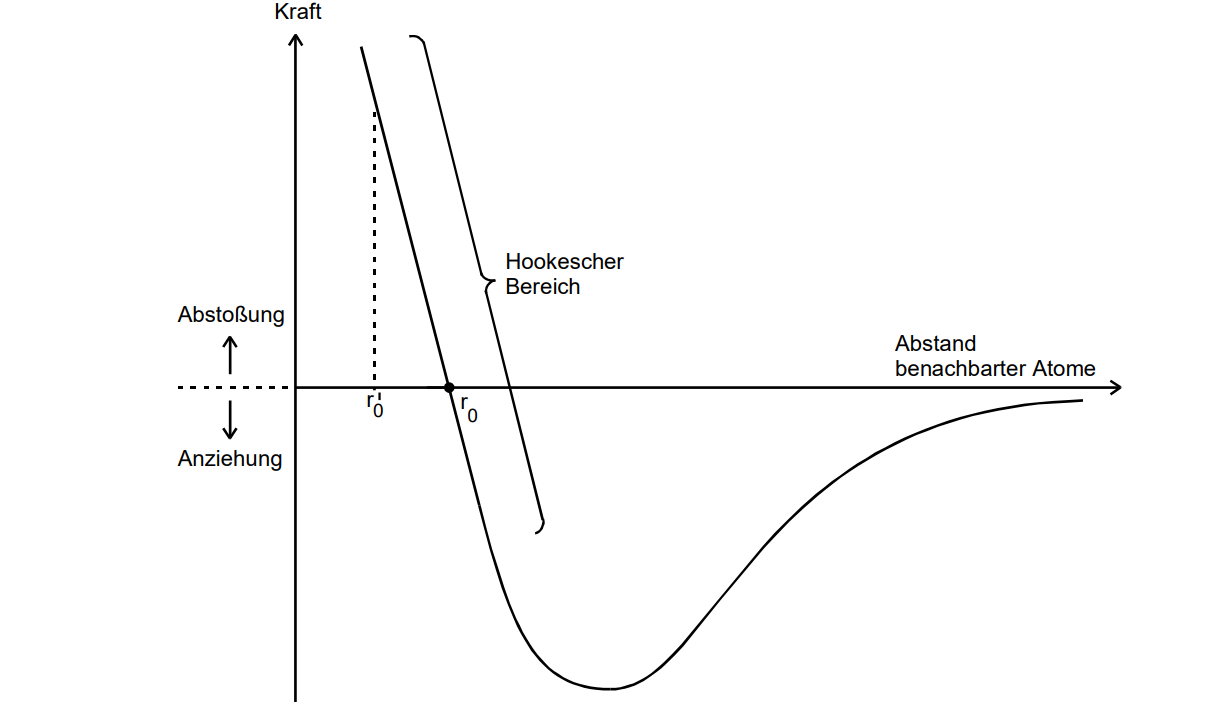
\includegraphics[width=\textwidth]{content/hook.png}
        \caption{Diagramm zur Veranschaulichung des Zusammenhanges zwischen einwirkender Kraft und Abstand der Atome im Kristallgitter \cite[93]{V102}.}
        \label{fig:hook}
    \end{figure}
    Das Hook'sche Gesetz gilt solange der Körper nur einer geringen Spannung $\sigma$ ausgesetzt ist, so dass nur eine elatische 
    Deformation vorliegt. In \autoref{fig:hook} wird dies als Hook'scher Bereich bezeichnet. Der Aufbau eines Körpers wird dabei
    als Kristallgitter betrachtet, in dem sich die Atome beziehugsweise Moleküle in einem Abstand $r$ in einem erlektrostatischen
    Gleichgewicht befinden. Durch Einwirkung einer äußeren Kraft verschiebt sich dieses Gleichgewicht und der Körper deformiert.
    Solange die Spannungen nicht zu groß sind, ist diese Deformation reversibel, sodass sich ein proportionaler Zusammenhang zwischen
    ergibt:
    \begin{equation}
    \label{eqn:hook}
        \sigma = E \frac {\Delta L} {L},
    \end{equation}     
    wobei $\frac {\Delta L}{L}$ die relative Längenänderung der Körpers und E das Elastizitätsmodul, auf welches in \autoref{sec:konstanten}
    näher eingegangen wird, bezeichnet.
    Insgesamt sind für die Beschreibung des Zusammenhanges zwischen Spannung und Deformation in einem Kristallgitter 36 Konstanten
    notwendig, durch Symmetrien veringert sich diese Zahl allerdings erheblich. 
    \subsection{Elastische Konstanten isotroper Körper}
    \label{sec:konstanten}
    Als isotrope Materialien werden Stoffe bezeichnet, deren Elastizitätskonstanten richtungsunabhängig sind. Hierdurch verringert
    sich die Zahl der Konstanten auf zwei. Ein solcher Körper wird auch bei der Messung verwendet.
    Die Konstanten sind einerseits das Schub- beziehugsweise Torsionsmodul $G$, welches die Gestaltselastizität beschreibt, 
    andererseit das Kompressionsmodul $Q$, welches die Volumenelastizität beschreibt. Hinzu kommen, aus Gründen der Zweckmäßigkeit
    noch das bereits erwähnte Elastizitätsmodul $E$ und die Poisson'sche Querkontraktionszahl $\mu$.
    $E$ beschreibt dabei die Längenänderung des Körpers unter Einfluss einer Normalspannung in Spannrichtung, während $\mu$ 
    die Längenänderung der Körpers senkrecht zur Normalspannung beschreibt. Letztere ist als 
    \begin{equation}
    \label{eqn:mu}
    \mu = - \frac{\Delta B}{B} \frac {L}{\Delta L}
    \end{equation}
    definiert. $\Delta B$ stellt dabei die Breitenänderung des Körpers da, was auch \autoref{fig:mu} verdeutlicht.
    \begin{figure}
        \centering
        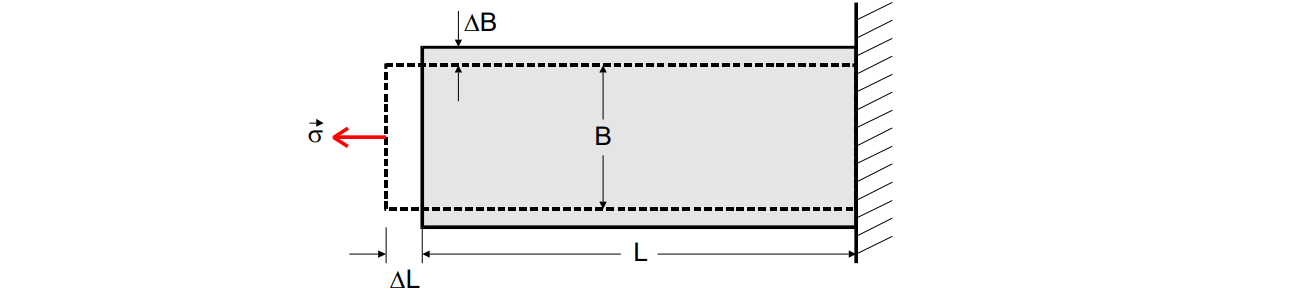
\includegraphics[width=\textwidth]{content/mu.png}
        \caption{Veranschaulichung der Querkontraktionszahl $\mu$ an einem gedrehten Stab \cite[94]{V102}.}
        \label{fig:mu}
    \end{figure}
    Weiterhin gelten folgende Zusammenhänge zwischen den Modulen:
    \begin{equation}
    \label{eqn:Zusammenhang1}
    E = 2 G (\mu + 1)
    \end{equation}
    und
    \begin{equation}
    \label{eqn:Zusammenhang2}
    E = 3 (1- 2 \mu) Q.
    \end{equation}
    Hieraus lassen sich die Module direkt berechnen, zu
    \begin{equation}
    \label{eqn:mubestimmen}
    \mu = \frac{E}{2G} -1
    \end{equation}
    und 
    \begin{equation}
    \label{eqn:Qbestimmen}
    Q = \frac{EG}{9G - 3E}
    \end{equation}
\subsection{Bestimmung des Schubmoduls $G$}
    \begin{figure}
        \centering
        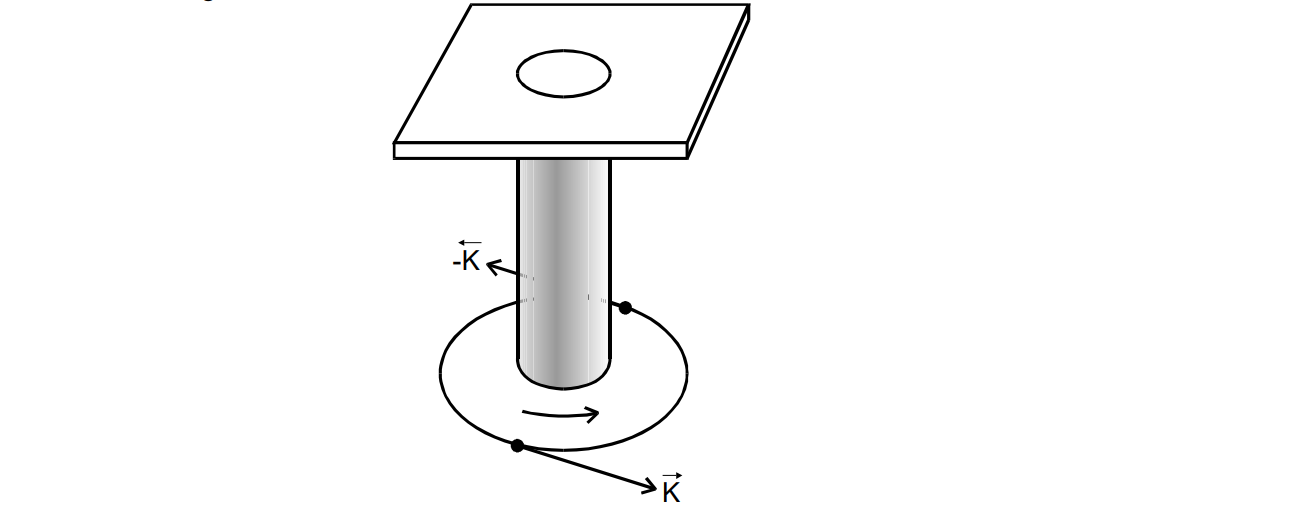
\includegraphics[width=\textwidth]{content/zylinder.png}
        \caption{Torsion an einem zylindrischen Stab \cite[96]{V102}.}
        \label{fig:zylinder}
    \end{figure}
    $G$ wird durch Betrachtung einer Torsion an einem zylindrischen Körper ermittelt.
    Wie in \autoref{fig:zylinder} zu sehen wirkt eine Kraft $K$ an zwei entgegengesetzten Punkten des kreisförmigen Körpers.  
    Das hierdurch entstehende Drehmoment $M$ ruft eine Torsion der unteren Zylinderfläche gegen die obere um den Winkel $\phi$ hervor.
    Bei der Berechnung von diesem, ist allerdings noch die Wirkung der Hebelarme, also dem Abstand der Massepunkte von der Drehachse,
    zu beachten, welcher aber über den Durchmesser des Körpers variert. Daraus ergibt sich die Notwendigkeit den Körper in Hohlzylinder
    mit infinitesimalen Dicken $dr$ und Radius $r$ zu zerlegen, wie in \autoref{fig:Hohlzylinder} zu sehen. Daraus ergibt sich 
    für jeden Hohlzylinder ein infinitesimales Drehmoment $dM$, welche anschließend über den Radius $R$ integriert werden.
    Mithilfe der Länge $L$ des Körpers und dem Scherungswinkel $\alpha$ ergibt sich zunächst unter Berücksichtigung des Hook'schen Gesetzes
    der Zusammenhang
    \begin{equation}
    \label{eqn:dM}
    dM = r G \alpha \, dF,
    \end{equation}
    womit sich das Drehmoment $M$ mit dem aus \autoref{fig:Hohlzylinder} ablesbaren 
    Winkelzusammenhang $ \alpha = \frac{r \phi}{L}$, ergibt zu 
    \begin{equation}
    \label{eqn:drehmoment}
    M = \int_0^{R} 2 \pi \frac{G}{L} r^3 \, dr = \frac {\pi}{2} G \frac {R^4}{L} \phi,
    \end{equation}
    woraus sich ein Proportionalitätsfaktor, die Richtgröße des Zylinders 
    \begin{equation}
    \label{eqn:richtgroesse}
    D := \frac{\pi G R^4}{2L},
    \end{equation}
    ableiten lässt.
    \begin{figure}
        \centering
        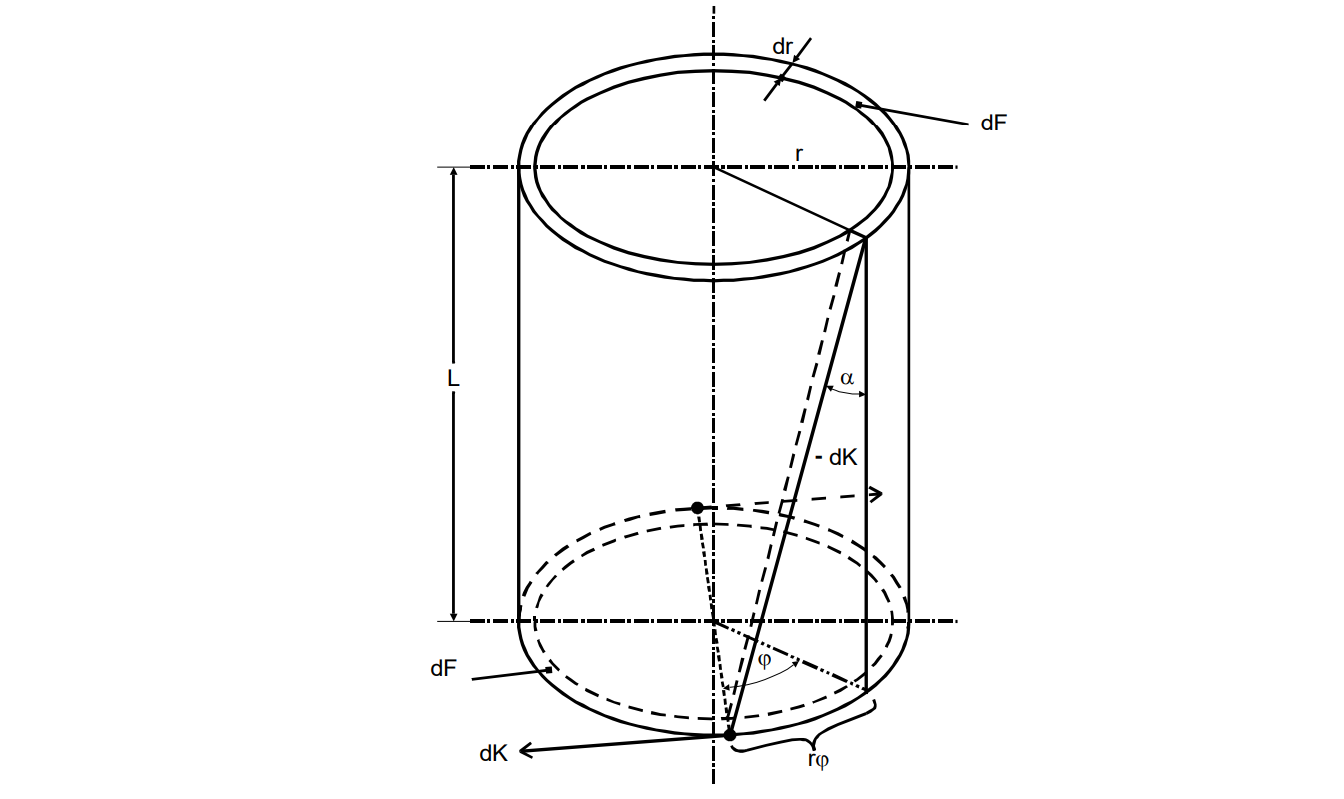
\includegraphics[width=\textwidth]{content/hohlzylinder.png}
        \caption{Schema zur Verdeutlichung des Zusammenhangs zwischen Drehmoment $M$ und Torsionswinkel $\phi$ an einem Zylinder \cite[97]{V102}.}
        \label{fig:Hohlzylinder}
    \end{figure}
    Hierbei kann es zur sogennanten elastischen Nachwirkung kommen.
    Sie beschreibt, dass ein Körper unter Spannung nicht direkt den entgültigen Deformationswert einstellt und umgekehrt beim 
    Verschwinden der Spannung nicht direkt in seine ursprüngliche Form zurückkehrt. Dies wird vermieden in dem eine sogenannte 
    dynamische Messmethode verwendet wird, bei dem die angelegte Kraft als periodische Funktion der Zeit auftritt.
    Experimentell betrachtet wird dies durch eine an einem Draht gehangene Kugel gelöst, welche ausgelenkt wird. Es greifen
    nun zwei entgegengesetzt wirkende Drehmomente, einerseits das des Drahtes welches mit Gleichung \eqref{eqn:drehmoment} dargestellt wird
    und andererseits das der Kugel, welches durch die Trägheit der Kugel $\Theta$ hervorgerufen wird, zu 
    \begin{equation}
    \label{eqn:drehmomentkugel}
    M_K = \Theta \frac{d^2\phi}{dt^2}.
    \end{equation}
    Aus den Gleichungen \eqref{eqn:drehmoment}, \eqref{eqn:richtgroesse} und \eqref{eqn:drehmomentkugel} lässt sich die Bewegungsgleichung
    als Differentialgleichung zweiter Ordnung formulieren:
    \begin{equation}
    \label{eqn:diffgleichung}
    D \phi + \Theta \frac{d^2\phi}{dt^2} = 0 .
    \end{equation}
    Durch Lösen mithilfe eines Cosinus-Ansatzes ergibt sich die Periodendauer $T$ zu
    \begin{equation}
    \label{eqn:periodendauer}
    T = 2 \pi \sqrt{\frac{\Theta}{D}}. 
    \end{equation}
    Das verwendete Trägheitsmoment $\Theta$ einer Kugel lässt sich aufgrund der Symetrien einer Kugel leicht herleiten, zu
    \begin{equation}
    \label{eqn:traegheit}
    \Theta = \frac {2}{5} m_K R_K^{2},
    \end{equation}
    wobei $m_K$ die Masse der Kugel und $R_K$ der Radius der Kugel ist,
    womit sich die Periodendauer aus Gleichung \eqref{eqn:periodendauer}, unter Zuhilfenahme der Definition von $D$ (Gleichung \eqref{eqn:richtgroesse}), vereinfachen lässt:
    \begin{equation}
    \label{eqn:periodendauer2}
    T = 2 \pi \sqrt{\frac{4 m_K R_K^{2} L}{5 \pi G R^4 }}.
    \end{equation}
    Somit lässt sich das Schubmodul $G$ schließlich über Glecihung \eqref{eqn:periodendauer2} bestimmen zu
    \begin{equation}
    \label{eqn:schubmodul}
    G = \frac{16 \pi m_K R_K^{2} L}{5 T^2 R^4}.
    \end{equation}
\subsection{Bestimmung des magnetischen Moments eines Permanentmagneten} 
    \begin{figure}
        \centering
        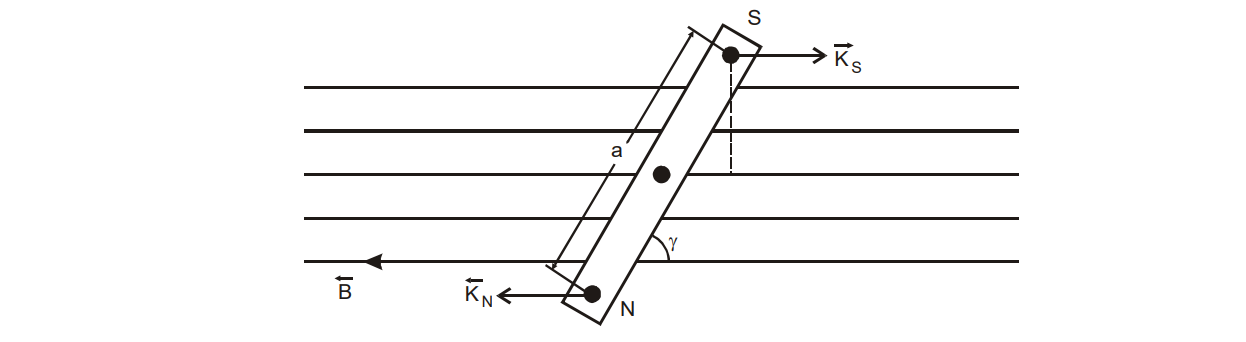
\includegraphics[width=\textwidth]{content/magnet.png}
        \caption{Permanentmagnet in einem äußeren, homogenen Magnetfeld \cite[103]{V102}.}
        \label{fig:magnet}
    \end{figure}
    Das magnetische Moment $\vec{m}$ ist definert durch die Polstärke $p$ und dem Abstand $\vec{a}$ zwichen den beiden Polen, zu
    \begin{equation}
    \label{eqn:magnetisch}
    \vec{m} = p \vec{a}.
    \end{equation}
    Durch anlegen eines homogenen Magnetfeldes wirken, wie in \autoref{fig:magnet} zu sehen, zwei Kräfte an den beiden Polen in 
    entgegengesetzter Richtung, sodass das ein Drehmoment $M_\text{mag}$ resultiert mit
    \begin{equation}
    \label{eqn:magdrehmoment}
    M_\text{mag} = p \vec{a} \times \vec{B} = \vec{m} \times \vec {B},
    \end{equation}
    dessen Betrag 
    \begin{equation}
    \label{eqn:betrag}
    M_\text{mag} = m B \sin \phi
    \end{equation}
    ist. Wenn derselbe Aufbau wie zur Bestimmung des Drehmomentes genutzt wird kann die Differentialgleichung \eqref{eqn:diffgleichung} zu
    \begin{equation}
    \label{eqn:magdiff}
    m B \sin \phi + D \phi + \Theta \frac{d^2\phi}{dt^2} = 0 
    \end{equation}
    aufgestellt werden.
    Lösen der Differentialgleichung ergibt eine Periodendauer von
    \begin{equation}
    \label{eqn:Periodendauermagnet}
    T_m = 2 \pi \sqrt{\frac{\Theta}{m B + D}} \iff m B + D := \Gamma = \frac {4 \pi^2 \Theta} {T_m^{2}}.
    \end{equation}

